% !TEX root = algo-quicksheet.tex
\chapter{Graph}

\section{Basic}
\runinhead{Graph representation.} $V$ for a vertex set with a map, mapping from vertex to its neighbors. The mapping relationship represents the edges $E$.
\begin{python}
V = defaultdict(list)
\end{python}

Convert a \pyinline{parent} array to graph, \pyinline{parent[i]} is the parent of node \pyinline{i}. 
\begin{python}
G = defaultdict(list)
for i, pi in enumerate(parent):
    G[pi].append(i)
\end{python}
\runinhead{Complexity.} Basic complexities:

\begin{table}

\begin{tabular}{lll}
\hline\noalign{\smallskip}
\textbf{Algorithm} & \textbf{Time}  & \textbf{Space}\\
\noalign{\smallskip}\hline\noalign{\smallskip}
dfs & $O(|E|)$ & $O(|V|), O(\text{longest path})$ \\
bfs & $O(|E|)$ & $O(|V|)$ \\
\noalign{\smallskip}\hline\noalign{\smallskip}
\end{tabular}

\caption{Time complexities}
\end{table}

\runinhead{Graph \& Tree.} For a undirected graph to be a tree, it needs to satisfied two conditions:
\begin{enumerate}
\item Acyclic
\item All connected
\end{enumerate}

\section{DFS}
\runinhead{Directed Graph.}
Use \pyinline{G  = defaultdict(dict)} to represent directed graph, so that later on the edge weight can be accessed as \pyinline{G[s][e]}. The \pyinline{s} start and \pyinline{e} end are the vertices, and \pyinline{G[s][e]} returns edge weight.

\runinhead{DFS.} DFS in directed graph:
\begin{python}
def dfs(self, G, s, e, path):
    if s not in G or e not in G:
        return -1
    if e in G[s]:
        return G[s][e]
    for nbr in G[s]:
        if nbr not in path:
            path.add(nbr)
            val = self.dfs(G, nbr, e, path)
            if val != -1.0:
                return val * G[s][nbr]
            path.remove(nbr)

    return -1
\end{python}

\runinhead{Number of Islands.} The most fundamental and classical problem.
\begin{python}
11000
11000
00100
00011
Answer: 3
\end{python}
\rih{Clue}:
\begin{enumerate}
\item Identify one island $\Ra$ dfs. 
\item To count multiple islands, need to mark/color the islands $\Ra$ visited.
\end{enumerate}
\begin{python}
class Solution:
  def __init__(self):
    self.dirs = [(-1, 0), (1, 0), (0, -1), (0, 1)]

  def numIslands(self, grid):
    cnt = 0
    m = len(grid)
    n = len(grid[0])
    visited = [
      [False for _ in range(n)]
      for _ in range(m)
    ]
    # visited = defaultdict(difaultdict(bool))
    for i in range(m):
      for j in range(n):
        if not visited[i][j] and grid[i][j] == "1":
          self.dfs(grid, i, j, visited)
          cnt += 1

    return cnt
\end{python}

\begin{python}
  def dfs(self, grid, i, j, visited):
    m = len(grid)
    n = len(grid[0])
    visited[i][j] = True

    for di, dj in self.dirs:
      I = i+di
      J = j+dj
      if 0 <= I < m and 0 <= J < n
        and not visited[I][J]
        and grid[I][J] == "1":
        self.dfs(grid, I, J, visited)
\end{python}
If the islands are constantly updating and the query for number of islands is called multiple times, need to use Union-Find (Section \ref{section:unionFind}) to reduce each query's complexity from $O(mn)$ to $O(\log mn)$.

Without updating, DFS itself is enough.

\section{BFS}
\subsection{BFS with Weights}
Each time, a query will add an edge from vertex $u$ to $v$, and find the shortest path from the $origin$ to $target$ after each update. 

\rih{Core clues}:
\begin{enumerate}
\item Forward vs. backward: \pyinline{dist} is the distance from origin, not to destination.
\item BFS updates the distance from the source of the newly added edge, not from the origin of the graph.
\item Shortest distance $\Ra$ 0-1 Dijsktra only nodes with \textit{improved} distance are added to the \textit{pending} queue.
\end{enumerate}
\begin{python}
def solve(self, G, dist, queries: List[Tuple])
    ret = []
    for u, v in queries:
        G[u].append(v)
        self.bfs(G, dist, u)  # from u
        ret.append(dist[~0])
    
    return ret
    
def bfs(self, G, dist, s):
    """
    Known origin and end destination
    """
    q = deque()
    q.append(s)
    while q:
        v = q.popleft()
        for nbr in G[v]:
            if dist[nbr] > dist[v] + 1:
                # It and its descendants require update
                dist[nbr] = dist[v] + 1
                q.append(nbr)
\end{python}
x\subsection{Transitive Closure}
\runinhead{Coverage closure in coordinates.} Given a list of bombs indexed by $(x,y)$ with a range $r$. The range of a bomb is defined as the area where its effect can be felt. The impact is circle. 

\rih{Core Clues:}
\begin{enumerate}
\item Given \textbf{pairwise} relations and query for \textbf{transitive} relations $\Ra$ Convert to a graph problem, two nodes are neighbors/linked if within range. To build the graph $G$, do pairwise checks $O(V^2)$.
\item Check max closure $\Ra$ dfs/bfs each node
\end{enumerate}

\begin{python}
def maximumDetonation(bombs):
    N = len(bombs)
    G = [[] for _ in range(N)]
    for i in range(N):
        x, y, r = bombs[i]
        for j in range(N):
            if i == j:
                continue
                
            x2, y2, _ = bombs[j]
            dx = x - x2
            dy = y - y2
            if dx * dx + dy * dy <= r * r:
                G[i].append(j)

    gmax = 1
    for i in range(N):
        visited = defaultdict(bool)
        visited[i] = True
        q = deque([i])

        cnt = 0
        while q:
            new_q = []
            for cur in q:
                cnt += 1
                for nbr in G[cur]:
                    if not visited[nbr]:
                        visited[nbr] = True
                        new_q.append(nbr)
            q = new_q

        gmax = max(gmax, cnt)

    return gmax
\end{python}
\runinhead{Evaluate Division.} Given an array of variable pairs equations and an array of real numbers values, where $equations_i = [a, b]$ and $values_i$ represent the equation $values_i = a / b$. 

Also given some queries, where $queries_i = [c, d]$ represents the jth query where you must find the answer for $c/d$.
\rih{Core Clues:}
\begin{enumerate}
\item Given pairwise relations and query for transitive relations $\Ra$ graph 
\item DFS for the queries
\end{enumerate}
\begin{python}
def calcEquation(self, equations, values, queries):
  # Build graph: G[u][v] = u / v
  G = defaultdict(dict)
  for (a, b), w in zip(equations, values):
    G[a][b] = w
    G[b][a] = 1.0 / w

  def dfs(s, e, acc, visited):
    if s == e:
      return acc
    
    visited[s] = True
    for nbr, w in G[s].items():
      if not visited[nbr]:
        ret = dfs(nbr, e, acc * w, visited)
        if ret != -1.0:
          return ret
          
    return -1.0
  
  rets = []
  for s, e in queries:
    ret = dfs(s, e, 1.0, defaultdict(bool))
    rets.append(ret)

  return rets
\end{python}
\subsection{Shortest Path \& Dijkstra}
\runinhead{Dijstrak.} Shortest path in the currently processing nodes $\Ra$ the queue holds the distance to the elements in a priority queue as shortest first. 
\runinhead{Swim in Rising Water.} Given an integer matrix $grid$ where each value $grid[i][j]$ represents the elevation at that point $(i, j)$. It starts raining, and water gradually rises over time. At time $t$, the water level is $t$, meaning any cell with elevation less than equal to $t$ is submerged or reachable. You can swim from a square to another 4-directionally adjacent square if and only if the elevation of both squares individually are at most $t$. You can swim infinite distances in zero time.

Start from top left, return the minimum time until you can reach the bottom right.

\rih{Core Clues:}
\begin{enumerate}
\item For any given path, the minimal time is the maximal elevation of a cell on the path
\item For any given cell, the minimal time to be on is the minimal of max elevations in possible paths containing the given cell. 
\item Min of maxes $\Ra$ Dijstrak
\item In Dijstrak implementation, we need priority queue $\Ra$ Heap
\end{enumerate}
\begin{python}
INF = sys.maxsize
dirs = [(1,0),(-1,0),(0,1),(0,-1)]
def swimInWater(self, grid):
  N = len(grid)
  # dist[i][j] = minimal of max elevations
  dists = [
    [INF for _ in range(N)] 
    for _ in range(N)
  ]
  dists[0][0] = grid[0][0]
  h = [(dists[0][0], 0, 0)]  # (distance_so_far, i, j)
  while h:
    dist, i, j = heapq.heappop(h)
    # first time pop is minimal
    if (i, j) == (N-1, N-1):
      return dist
    
    # skip outdated minimal distance
    if dist > dists[i][j]:
      continue

    for di, dj in dirs:
      I, J = i + di, j + dj
      if 0 <= I < N and 0 <= J < N:
        # transfer function from i,j to I,J
        nxt_dist = max(dist, grid[I][J])
        if nxt_dist < dists[I][J]:
          dists[I][J] = nxt_dist
          heapq.heappush(h, (nxt_dist, I, J))

  return dists[~0][~0] # redundant
\end{python}

Alternatively, we can binary search the time. The predicate is whether we can BFS to the target. 
\begin{python}
def bfs(self, grid, t) -> bool:
  N = len(grid)
  if grid[0][0] > t: 
    return False
  
  visited = defaultdict(lambda: defaultdict(bool))
  q = [(0,0)]
  visited[0][0] = True
  while q:
    new_q = []
    for i, j in q:
      if (i, j) == (N-1, N-1):
        return True
      
      for di, dj in dirs:
        I, J = i + di, j + dj
        if 0 <= I < N and 0 <= J < N \
        and not visited[I][J] and grid[I][J] <= t:
          new_q.append((I, J))
          visited[I][J] = True
    q = new_q
    
  return False

def swimInWater(self, grid):
  N = len(grid)
  lo = 0
  hi = N*N
  while lo < hi:
    mid = (lo + hi) // 2
    if self.bfs(grid, mid):
      hi = mid
    else:
      lo = mid + 1

  return lo
\end{python}
\runinhead{0-1 Dijstrak.} Only two buckets of priorities: $d$ or $d+1$ $\Ra$ the queue always pop from the left the lowest weighted candidate $\Ra$ add the new candidate to the deque with a larger weight $\Ra$ checking the compared to decide append left or right. 

Time compexlity: visit every node and every edge $\Ra O(|V| + |E|)$. 

\runinhead{Minimum cost to form a valid path.} A valid path in the grid is a path that starts from $(0, 0)$ and ends at the $(\sim 0, \sim 0)$ following the signs on the grid. The sign is in $A_{i,j}$: 1 right, 2 left, 3 down, 4 up. 

\rih{Core Clues:}
\begin{enumerate}
\item Cost of changing signs $\Ra$ weights in graph 
\item Minimum cost $\Ra$ minimum distance $\Ra$ BFS $\Ra$ 0-1 Dijstrak
\end{enumerate}
\begin{python}
def minCost(self, A):
    dirs = {
        1: (0, 1), 
        2: (0, -1), 
        3: (1, 0), 
        4: (-1, 0),
    }
    
    M, N = len(A), len(A[0])
    W = [
        [sys.maxsize for _ in range(N)]
        for _ in range(M)
    ]
    W[0][0] = 0
    
    q = deque()
    while q:
        i, j = q.popleft()
        for orient, (di, dj) in dirs.items():
            I = i + di
            J = j + dj
            if 0 <= I < M and 0 <= J < N:
                # delta weight
                dw = 0 if A[i][j] == orient else 1
                if W[i][j] + dw < W[I][J]:
                    W[I][J] = W[i][j] + dw
                    if dw == 0:
                        q.appendleft((I, J))
                    else:
                        q.append((I, J))
    return W[~0][~0]
\end{python}
\subsection{Multi-source BFS}

BFS goes through the vertices level by level in a queue. 

Distance can be targetedly defined to solve the problem. BFS can start with a set of vertices in abstract level of distance, not necessarily neighboring vertices.

\runinhead{Shortest distance to nearest origins.} Given $-1$ denotes obstacles, $0$ denotes targets, calculate all other vertices' Manhattan distance to its nearest target.
\rih{Core clues:}
\begin{enumerate}
\item Shortest distance $\Ra$ bfs
\item Multiple source/origins $\Ra$ multi-source bfs. 
\end{enumerate}
$$
\begin{bmatrix}
\infty & -1 & 0 & \infty \\
\infty & \infty & \infty & -1 \\
\infty & -1 & \infty & -1 \\
0 & -1 & \infty & \infty \\
\end{bmatrix}
$$

Then it is calculated as:
$$
\begin{bmatrix}
3 & -1 & 0 & 1 \\
2 & 2 & 1 & -1 \\
1 & -1 & 2 & -1 \\
0 & -1 & 3 & 4 \\
\end{bmatrix}
$$

\begin{python}
self.dirs = [(-1, 0), (1, 0), (0, -1), (0, 1)]

def wallsAndGates(self, mat):
  M = len(mat)
  N = len(mat[0])
  q = [
    (i, j) 
    for i in range(M)
    for j in range(N)
    if mat[i][j] == 0
  ]
  for i, j in q:
    for di, dj in self.dirs:
      I, J = i+di, j+dj
      if 0 <= I < m and 0 <= J < n 
        and mat[I][J] > mat[i][j]+1:  # test distance
        mat[I][J] = mat[i][j]+1  # not min(...)
        q.append((I, J))
\end{python}

\runinhead{Shortest bridge of two islands.} Given an binary matrix $A$ where 1 represents land and 0 represents water. Return the smallest number of 0's you must flip to connect the two islands.

\rih{Core Clues:}
\begin{enumerate}
\item Two islands $\Ra$ coloring $\Ra$ since only two islands $\Ra$ color one of them is enough
\item The points on the island edge are sources $\Ra$ multi-source BFS 
\item No harm to treat inland points as sources. 
\end{enumerate}
\begin{python}
def shortestBridge(self, A) -> int:
  dirs = [(-1, 0), (1, 0), (0, -1), (0, 1)]
  M, N = len(A), len(A[0])
  inbound = lambda i, j: 0 <= i < M and 0 <= j < N

  def dfs(i, j, visited, color):
    A[i][j] = color
    visited[i][j] = True
    
    for di, dj in dirs:
      I = i + di
      J = j + dj
      if inbound(I, J) and A[I][J] == 1 \
        and not visited[I][J]:
        dfs(I, J)

  # Find first island and color it
  def color():
    visited = defaultdict(defaultdict(bool))
    for i in range(M):
      for j in range(N):
        if A[i][j] == 1 and not visited[i][j]:
          dfs(i, j, visited, color=2)
          return
  color()
  
  # Multi-source BFS
  q = deque()
  for i in range(M):
    for j in range(N):
      if A[i][j] == 2:
        q.append((i, j))
  step = 0 
  visited = defaultdict(defaultdict(bool))
  while q:
    new_q = []
    for i, j in q:
      for di, dj in dirs:
        I = i + di
        J = j + dj
        if inbound(I, J) and not visited[I][J]:
          if A[I][J] == 1:
            return step  # reached 1's
          if A[I][J] == 0:
            new_q.append((I, J))
            visited[I][J] = True
    q = new_q
    step += 1

  return -1
\end{python}
\runinhead{Escape the Spreading Fire.} Given a matrix $grid$. Each cell has one of three values:
\begin{itemize}
\item 0 represents grass
\item 1 represents fire
\item 2 represents a wall that you and fire cannot pass through
\end{itemize}
Starting from top-left cell to travel to the safehouse at the bottom-right cell. Every minute, you may move to an adjacent grass cell. After your move, every fire cell will spread to all adjacent cells that are not walls.

Return the maximum wait time that you can stay in your initial position before moving.

Note that even if the fire spreads to the safehouse immediately after you have reached it, it will be counted as safe.

\rih{Core Clues:}
\begin{enumerate}
\item Every minute is a tick. 
\item Spreading filre $\Ra$ multi-source BFS to calculate the fire arrival time for each cell
\item Reachable from start to end? $\Ra$ BFS from start to calculate travel time.
\item Numeric binary search for the maximum wait time. 
\item Note that: Normal cells: must have travelTime $<$ fireTime. Goal cell: travelTime $\leq$ fireTime.
\end{enumerate}
\begin{python}
DIRS = [(-1, 0), (1, 0), (0, -1), (0, 1)]

class Solution:
  def maximumMinutes(self, grid) -> int:
    M, N = len(grid), len(grid[0])
    # 1) Multi-source BFS for fire arrival times
    fire = [
      [sys.maxsize for _ in range(N)] 
      for _ in range(M)
    ]
    q = []
    for i in range(M):
      for j in range(N):
        if grid[i][j] == 1:  # fire source
          fire[i][j] = 0
          q.append((i, j))

    while q:
      new_q = []
      for i, j in q:
        t = fire[i][j]
        for di, dj in DIRS:
          I, J = i+di, j+dj
          if 0 <= I < M and 0 <= J < N and grid[I][J] != 2:
            if fire[I][J] > t + 1:
              fire[I][J] = t + 1
              new_q.append((I, J))
      q = new_q
	
    # 2) reachable after wait for T
    def reachable(T) -> bool:
      if fire[0][0] <= T:
        return False

      q = [(0, 0, T)]  # (r, c, time)
      visited = defaultdict(lambda: defaultdict(bool))
      visited[0][0] = True
      while q:
        new_q = []
        for i, j, t in q:
          if (i, j) == (M-1, N-1):
            return t <= fire[i][j]

          for di, dj in DIRS:
            I, J = i + di, j + dj
            if 0 <= I < M and 0 <= J < N \
              and grid[I][J] != 2 and not visited[I][J]:
              nt = t + 1
              if (I, J) != (M-1, N-1):
                if nt < fire[I][J]:
                  new_q.append((I, J, nt))
                  visited[I][J] = True
              else:
                # edge case
                return nt <= fire[I][J]
        q = new_q

      return False

    # 3) Binary search the maximum feasible wait
    lo, hi = 0, 10**9 + 1
    ret = -1
    while lo < hi:
      mid = (lo + hi) // 2
      if reachable(mid):
        ret = mid
        lo = mid + 1
      else:
        hi = mid

    return ret
\end{python}

\section{Detect Cycle}
\begin{enumerate}
\item Circle in current dfs? $\Ra$ \pythoninline{path} represents the current path, and it is reset/pop after a dfs. \pyinline{path} is the \pyinline{rec_stk} that represents the \textbf{recursion stack} of the dfs. 
\item Next node connect back to the current node $\Ra$ 
\begin{enumerate}
\item For directed graph:
\begin{enumerate}
\item Should dfs for all neighbors except for vertices in \pythoninline{visited}, to avoid revisiting. For example, avoid revisiting A, B when start from C in the graph, and A, B have already been visited $C \rightarrow A \rightarrow B$. \pythoninline{visited} should be updated only in the \textbf{end} of the dfs.
\item Otherwise excluding predecessor \pythoninline{pi} is wrong considering the case of $A \leftrightarrow B$
\end{enumerate}
\item For \pinkhl{undirected} graph:
\begin{enumerate}
\item Besides \pyinline{cur}, we should track \hl{predecessor} \pyinline{pi}. We should dfs for all neighbors except for the \textbf{predecessor} \pythoninline{pi}. $A-B$.
\item Excluding neighbors in \pythoninline{visited} is redundant, due to \pyinline{pi}. But it is okay to double check \pythoninline{visited}.
\end{enumerate}
\end{enumerate}
\end{enumerate}

\runinhead{Directed Graph.}
Detect cycles (any) in directed graph.

\begin{python}
def dfs(self, G, v, visited, path) -> bool:
  if v in path:
    return False

  path.add(v)
  for nbr in G[v]:
    if nbr not in visited:
      if not self.dfs(G, nbr, visited, path):
        return False

  path.remove(v)
  visited.add(v)
  return True
\end{python}
\runinhead{Undirected Graph.}
Detect cycles (any) in undirected graph.

\begin{python}
def dfs(self, G, cur, pi, visited, path):
  if cur in path:
    return False

  path.add(cur)
  for nbr in G[cur]:
    if nbr != pi:  # nbr not in visited
      if not self.dfs(G, nbr, cur, visited, path):
        return False

  path.remove(cur)
  visited.add(cur)
  return True
\end{python}

Alternatively, we can collapose $path$ into $visited$ using coloring:
\begin{python}
visited[u] = 0  # unvisited
visited[u] = 1  # visiting
visited[u] = 2  # visited
\end{python}

\section{Bipartite Graph}
A bipartite graph is a graph whose vertices can be split into two disjoint sets $U$ and $V$ such that every edge goes between the sets (none within the same set).
\begin{center}
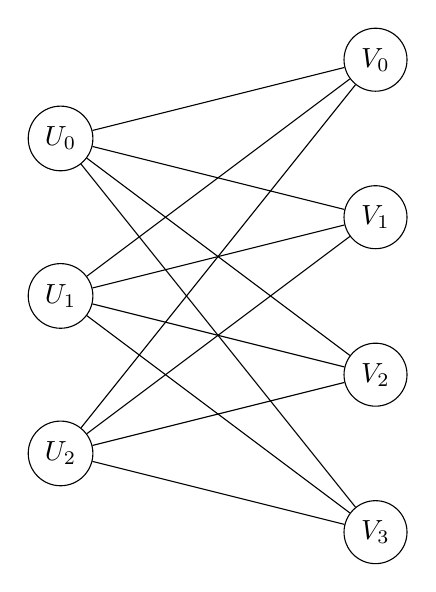
\begin{tikzpicture}[every node/.style={circle, draw, minimum size=8mm}]
  % Left side (3 nodes)
  \node (U0) at (0,2) {$U_0$};
  \node (U1) at (0,0) {$U_1$};
  \node (U2) at (0,-2) {$U_2$};

  % Right side (4 nodes)
  \node (V0) at (4,3) {$V_0$};
  \node (V1) at (4,1) {$V_1$};
  \node (V2) at (4,-1) {$V_2$};
  \node (V3) at (4,-3) {$V_3$};

  % Edges (connect every left to every right)
  \foreach \i in {0,1,2} {
    \foreach \j in {0,1,2,3} {
      \draw (U\i) -- (V\j);
    }
  }
\end{tikzpicture}
\end{center}
\runinhead{Bus routes.} Given an array $routes$ representing bus routes where $routes_i$ is a bus route that the i-th bus loops at bus stops forever. For example, if $routes_i = [1, 5, 7]$. 

Find the least number of buses you must take to travel from $source$ to $target$.

\rih{Core clues:}
\begin{enumerate}
\item Bus stops are connected through routes, not directly $\Ra$ bipartite graph as stops $U$, and routes $V$. 
\item From $source$, we visisted multiple $u$ through the bus route $v$ $\Ra$ multi-source BFS
\end{enumerate}


\begin{python}
def numBusesToDestination(self, routes, source, target):
  # graph of stops U, graph of routes V
  U = defaultdict(set)
  V = defaultdict(set)
  for v, us in enumerate(routes):
    for u in us:
      U[u].add(v)
      V[v].add(u)

  # BFS
  visited_U = defaultdict(bool)
  visited_V = defaultdict(bool)
  visited_U[source] = True
  for v in U[source]:
    visited_V[v] = True

  v_q = []
  for v in U[source]:
    v_q.append(v)

  step = 1
  while v_q:
    new_v_q = []
    for v in v_q:
      if target in V[v]:
        return step

      for u in V[v]:
        if not visited_U[u]:
          visited_U[u] = True
          for nxt_v in U[u]:
            if not visited_V[nxt_v]:
              new_v_q.append(nxt_v)
              visited_V[nxt_v] = True

    v_q = new_v_q
    step += 1

  return -1
\end{python}
\section{Paths}
\subsection{Visit Every Edge Once $\forall e$ - Euler Path} 
An Eulerian path is a path in a graph which visits every edge exactly once ($\forall e \in E$). Vertices can be repeated.

Hierholzer's algorithm to find an Euler path in a graph. The graph must be \textbf{directed} graph.

\runinhead{Core clue.}
\begin{enumerate}
\item The algorithm exhaustively visit all the edges during the dfs. 
\item \rih{Post-order traversal}. Dfs a vertex $v$'s all neighbors and path. After this, process  this current vertex $v$ by \pyinline{appendleft}. 
\item How to avoid circle?
\begin{enumerate}
\item Checking predecessor $\pi$? Not sufficient, since $\pi$ can be reached again if circle. 
\item Visited? $\Ra$ We must \textbf{remove} the edge $e$ after being visited. 
\item Or we can record the visited edge $e=(u,v)$ in a dict \pyinline{visited}, but only if no duplicates in $E$; otherwise we must use a counter and it becomes the same as removing.
\end{enumerate}
\end{enumerate}
\begin{center}
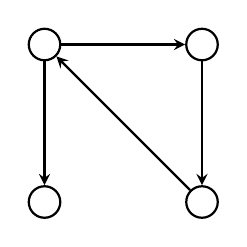
\begin{tikzpicture}[->,>=stealth, node distance=2cm, thick]
  \tikzstyle{every node}=[circle, draw, minimum size=0.4cm]

  \node (A) at (0, 2) {};
  \node (B) at (2, 2) {};
  \node (C) at (2, 0) {};
  \node (D) at (0, 0) {};

  \path
    (A) edge (B)
    (B) edge (C)
    (C) edge (A)
    (A) edge (D);

\end{tikzpicture}
\end{center}

Sorted for lexical order. 
\begin{python}
def findItinerary(self, tickets):
    G = defaultdict(deque)
    for s, e in tickets:
        G[s].append(e)
    
    for s, l in G.items():
        G[s] = deque(sorted(l))
    
    ret = deque()
    self.dfs(G, "JFK", ret)
    return list(ret)

def dfs(self, G, cur, ret):
    while G[cur]:
        # need to remove the edge after visting
      	# thus not for-loop
        nbr = G[cur].popleft()
        self.dfs(G, nbr, ret)
    
    ret.appendleft(cur)
\end{python}

Alternatively, instead of using sorted list, using \pyinline{heapq}.

\begin{python}
def findItinerary(self, tickets):
    G = defaultdict(list)
    for s, e in tickets:
        heapq.heappush(G[s], e)  # heap lexical order

    ret = deque()
    self.dfs(G, 'JFK', ret)
    return list(ret)

def dfs(self, G, cur, ret):
    while G[cur]:
        # need to remove the edge after visting
        nbr = heapq.heappop(G[cur])
        self.dfs(G, nbr, ret)

    ret.appendleft(cur)
\end{python}

\subsection{Vist Every Vertex Once $\forall v$ - Hamiltonian Path, NP} 

A Hamiltonian path is a path in a graph which visits every vertex exactly once ($\forall v \in V$). This problem is proved to be NP.

\section{Topological Sorting}
For a graph $G=\{V, E\}$, if $A \rightarrow B $, then $A$ is before $B$ in the ordered list.
\subsection{Algorithm}
\rih{Core clues}:
\begin{enumerate}
\item \textbf{DFS neighbors first}. For a given vertex $v$, if the neighbors of current node is  $\neg$visited, then dfs the neighbors
\item \textbf{Process current node}. After visiting all the neighbors, then visit the current node $v$ and push it to the result queue \pyinline{appendleft}.
\item \textbf{Acyclic}. Need to detect cycle using $path$; thus the dfs need to construct result queue $ret$ and detect cycle simultaneously - by using two sets: $visited$ and $path$. The $path$ can also be named as \pyinline{rec_stk} to represent \hl{recursion stack} in DFS. 
\end{enumerate}
Notice:
\begin{enumerate}
\item Need to check ascending order or descending order.
\end{enumerate}


\begin{figure}[h!]
  \centering
  \begin{tikzpicture}[
      scale=0.7,
	  transform shape, 
      node/.style={circle, draw, minimum size=1cm},
      ->, >=Stealth
    ]

    % Nodes
    \node[node] (0) at (0,0) {0};
    \node[node] (1) at (2,1.5) {1};
    \node[node] (2) at (2,-1.5) {2};
    \node[node] (3) at (4,-1.5) {3};
    \node[node] (4) at (6,-0.5) {4};
    \node[node] (5) at (4,0.5) {5};
    \node[node] (6) at (3,3) {6};

    % Edges
    \draw (0) -- (1);
    \draw (0) -- (2);
    \draw (1) -- (2);
    \draw (1) -- (5);
    \draw (2) -- (3);
    \draw (5) -- (3);
    \draw (5) -- (4);
    \draw (6) -- (1);
    \draw (6) -- (5);

  \end{tikzpicture}
  \begin{tikzpicture}[
  	  scale=0.6,
	  transform shape, 
      node/.style   ={circle, draw, minimum size=1cm},
      ->, >=Stealth
    ]

    %---------------- Nodes ----------------%
    %\foreach \i in {0,...,6}{
    %	\node[node] (n\i) at (\i*2,0) {\i};
	%}
	\node[node] (n0) at (0,0)  {0};
    \node[node] (n6) at (2,0)  {6};
    \node[node] (n1) at (4,0)  {1};
    \node[node] (n5) at (6,0)  {5};
    \node[node] (n4) at (8,0)  {4};
    \node[node] (n2) at (10,0) {2};
    \node[node] (n3) at (12,0) {3};

	
    %---------------- Arrows ----------------%
    % black
    \draw[->, black, bend left=25] (n0) to (n1);
    \draw[->, black, bend left=55] (n0) to (n2);

    % blue
    \draw[->, blue, bend left=25]  (n6) to (n1);
    \draw[->, blue, bend left=45]  (n6) to (n5);

    % green
    \draw[->, green!70!black, bend left=25] (n1) to (n5);
    \draw[->, green!70!black, bend left=55] (n1) to (n2);

    % yellow
    \draw[->, yellow!80!black, bend left=25] (n5) to (n4);
    \draw[->, yellow!80!black, bend left=55] (n5) to (n3);

    % red
    \draw[->, red!70!black, bend left=25]   (n2) to (n3);
    \draw[<-] (0,-1) -- (12,-1);
    % Caption centred under the arrow
    \node[below] at (6,-1) {build direction};	
    
  \end{tikzpicture}
  \caption{Unsorted DAG to Topologically Sorted}
  \label{fig:dag}
\end{figure}

\begin{python}
from collections import deque

def topological_sort(self, V):
  visited = set()
  ret = deque()

  for v in V.keys():
    if v not in visited:
      if not self.dfs_topo(V, v, visited, set(), ret):
        return []  # contains cycle

  return list(ret)

# return whether the current path is acyclic
def dfs_topo(self, V, v, visited, path, ret) -> bool:
  if v in path:  # cycle
    return False

  path.add(v)
  for nbr in V[v]:
    if nbr not in visited:
      if not self.dfs_topo(V, nbr, visited, path, ret):
        return False

  path.remove(v)
  visited.add(v)
  ret.appendleft(v)
  return True
\end{python}
Alternatively, we can encode \pyinline{path} into \pyinline{visited}, i.e. coloring. 
\begin{python}
# encode the visited using 0, 1, 2
def dfs_topo(
  self, 
  G: Dict[int, List[int]], 
  u: int, 
  visited: Dict[int, int],
  ret: Deque,
) -> bool:
  """
  Topological sort
  G = defaultdict(list)
  visited = defaultdict(int) 
  # 0 not visited, 1 visiting, 2 visited

  pre-condition: u is not visited (0)
  """
  visited[u] = 1
  for nbr in G[u]:
    if visited[nbr] == 1:
      return False
    if visited[nbr] == 0:
      if not self.topo_dfs(G, nbr, visited, ret):
        return False

  visited[u] = 2
  ret.appendleft(u)  # visit larger first
  return True
\end{python}
The time complexity of topological sorting is $O(|E|+|V|)$ since it needs to goes to every edges and every vertices. 

\subsection{Applications}
\begin{enumerate}
\item Course scheduling problem with pre-requisite.
\item In a tree, find the closest ancestor $y$ of $x$ s.t. sastisfying some predicate. 
\end{enumerate}

In a tree, find the closest ancestor $y$ of node $x$ that has the same value $s[x] = s[y]$ and set $x$ parent to $y$. 

\rih{Core clues}:
\begin{enumerate}
\item Naively dfs updating the tree results in TLE of $O(N^2)$. Thus we need to do a topological dfs on the tree for $O(N)$.
\item During topological dfs, the recursion stack $path$ holds \textbf{extra} information. The $path$ holds the map of a stack of ancestors with a given value, with the last one as the closest. 
\end{enumerate}
\begin{python}
def topo(self, G, cur, path: Dict[List], parents, s):
    # topological dfs
    val = s[cur]
    if len(path[val]) > 0:
        pi = path[val][~0]
        parent[cur] = pi
    
    path[val].append(cur)
    for v in G[cur]:
        self.topo(G, v, path, parent, s)
    path[val].pop()
\end{python}

\runinhead{Alien Dictionary}. Given a list of words, and they are lexicially sorted. Return the lexical order of chars. Input: \pyinline{words = ["wrt","wrf","er","ett","rftt"]}, Output: \pyinline{"wertf"}.
\rih{Core Clues}:
\begin{enumerate}
\item Relax the problem: single char $\Ra$ topo sort 
\item The difficult parts lie in how to construct the graph $G$.
\item Multi chars: first char diff btw two words tells the \textbf{relative} order 
\item When build the graph G, we need to check acyclic 
\item When topo sort, we need to check acyclic
\end{enumerate}
\begin{python}

class Solution:
  def construct_graph(self, words: List[str]):
    G = defaultdict(set)  # use set to avoid duplicate edges

    for w in words:
      for c in w:
        G[c]

    # compare two words 
    for i in range(len(words) - 1):
      w1, w2 = words[i], words[i + 1]

      # invalid if w2 is a strict prefix of w1
      if len(w1) > len(w2) and w1.startswith(w2):
        return G, False

      for c1, c2 in zip(w1, w2):
        # first diffs
        if c1 != c2:
          if c2 not in G[c1]:
            G[c1].add(c2)
          break

    return G, True

  def topo_dfs(self, G, u, visited, ret) -> bool:
    visited[u] = 1
    for nbr in G[u]:
      if visited[nbr] == 1:
        return False  # not acyclic
      if visited[nbr] == 0:
        if not self.topo_dfs(G, nbr, visited, ret):
          return False

    visited[u] = 2
    ret.appendleft(u)
    return True
  
  def alienOrder(self, words) -> str:
    G, acylic = self.construct_graph(words)
    if not acylic:
      return ""

    # coloring: # 0 not visited, 1 visiting, 2 visited
    ret = deque()
    visited = defaultdict(int)

    for u in G.keys():
      if visited[u] == 0:
        if not self.topo_dfs(G, u, visited, ret):
          return ""

    return "".join(ret)
\end{python}

\section{Union-Find}\label{section:unionFind}
\subsection{Simplified Union Find}
Simplified code with unbalanced size. Union-find and disjoint set are used interchangeably. Union-find emphasizes on algorithm while disjoint set emphasizes on data structure.

\rih{Core clues:}
\begin{enumerate}
\item \textbf{$\pi$ array}:an array to store each item's predecessor pi. The predecessor are lazily updated to its ancestor. 
\item When \pyinline{x == pi[x]}, then \pyinline{x} is the ancestor (i.e. root). Don't introduce a dummy node \pyinline{-1}. Self-equaling is enough.
\item Otherwise, \pyinline{pi[x] = find(pi[x])}, recursively. Need to find \pyinline{x}'s \pyinline{pi} to make progress in the recursive function.
\item When $union$, find the ancestors of both nodes, and set one's ancestor to the other's.  
\item Lazily init \pyinline{pi[x]} during $find$ since $find$ is invoked inside $union$. 
\end{enumerate}
\begin{python}
class UnionFind:
    def __init__(self):
        self.pi = {}

    def union(self, x, y):
        pi_x = self.find(x)
        pi_y = self.find(y)
        self.pi[pi_y] = pi_x

    # find root
    def find(self, x):
        # lazy init
        if x not in self.pi:
          self.pi[x] = x
          return x
        
        # path compression
        pi = self.pi[x]
        if x != pi:
          root = self.find(pi)
          self.pi[x] = root
        return self.pi[x]
\end{python}

Note, for the final counting of component. Need to do a final find on all nodes to
update the ancestor.
\begin{python}
component_cnt = len(set(
    uf.find(x)
    for x in uf.pi.keys()
))
\end{python}
Alternatively using iterative:
\begin{python}
def find(self, x):
    # lazy init
    if x not in self.pi:
        self.pi[x] = x
        return x

    cur = x
    while cur != self.pi[cur]:
        cur = self.pi[cur]

    self.pi[x] = cur
    return cur
\end{python}
Note that it only updates \pyinline{self.pi[x]}, so nodes between \pyinline{x} and the root aren’t compressed. That’s correct but less efficient than full compression.

Improvements:
\begin{enumerate}
\item Weighting: size-baladnced tree
\item Path Compression.
\end{enumerate}
\subsection{Optimized Union Find}
Weighted union-find with path compression.\\
\rih{Core clues:}
\begin{enumerate}
\item \textbf{$\pi$ array}: predecessor pi.
\item \textbf{Size-balanced}: merge the tree according to the size to maintain balance.
\item \textbf{Path compression}: Make the ptr in $\pi$ array to point to its root rather than its immediate parent.
\end{enumerate}
\begin{figure}[]
\centering
\subfloat{\includegraphics[width=0.9\linewidth]{uf}}
\caption{Weighted union find traces, on every union operation}
\label{fig:union_find}
\end{figure}

\begin{python}
class UnionFind:  # or DisjointSet
  def __init__(self):
    self.pi = {}  # item -> pi
    self.sz = {}  # root -> size

  def find(self, x):
    """path compression"""
    if x not in self.pi:
      self.pi[x] = x
      self.sz[x] = 1
      return x

    pi = self.pi[x]
    if x != pi:
      root = self.find(pi)
      self.pi[x] = root
    return self.pi[x]

  def union(self, x, y):
    pi_x = self.find(x)
    pi_y = self.find(y)

    if pi_x != pi_y:
      if self.sz[pi_x] > self.sz[pi_y]:
        pi_x, pi_y = pi_y, pi_x
        # size balancing, remove the smaller one
      self.pi[pi_x] = pi_y
      self.sz[pi_y] += self.sz[pi_x]
      del self.sz[pi_x]

  def is_union(self, x, y):
    if x not in self.pi or y not in self.pi:
      return False
    return self.find(x) == self.find(y)

  def __len__(self):
    """number of sets"""
    return len(self.sz)  # only root nodes have size
\end{python}

\subsection{Complexity}
$m$ union-find with $n$ objects: $O(n)+m O(\lg n)$

\subsection{MST}
Minimum spanning tree. A minimum spanning tree (MST) is a subset of a graph's edges that connects all the vertices while minimizing the total edge weight.

\runinhead{Kruskal's algorithm.} Greedily add minimal edge. 

\rih{Core clues:}
\begin{enumerate}
\item Vertices $v \in V$ are divided into different sets
\item \textbf{Greedily} use min edges to unionize the sets if not in the same union, by sorting the edge weights
\item Terminates when $\forall v\in V$ are in the same set.
\end{enumerate}
\textbf{Code:}
\begin{python}[mathescape]
def kruskal(G):
  ret = []
  uf = UnionFind()
  for v in G.V:
    uf.add(v)

  G.E.sort()  # sort by weights
  for u, v in G.E:
    if not uf.is_union(u, v):
      A.append((u, v))
      uf.union(u, v)
\end{python}
Complexity: $O(|E|\log |E|)$.

